\subsection{Расчет отчислений}
В рамках данной работы был реализован механизм расчета отчисления в соответствии с поставленными требованиями.
По причине того, что в случае большого количества записей в таблицах, связанных со статистикой Live, расчет отчислений
может длиться до нескольких минут, было принято решение реализовать его в виде фоновой задачи.
Большая часть бизнес-логики алгоритма реализована в рамках классов модели предметной области, более подробно реализация
рассмотрена в диаграмме последовательности на рис. \ref{gr:calc_deduct}

\begin{figure}[!ht]
\begin{center}
\vspace{-0.4cm}
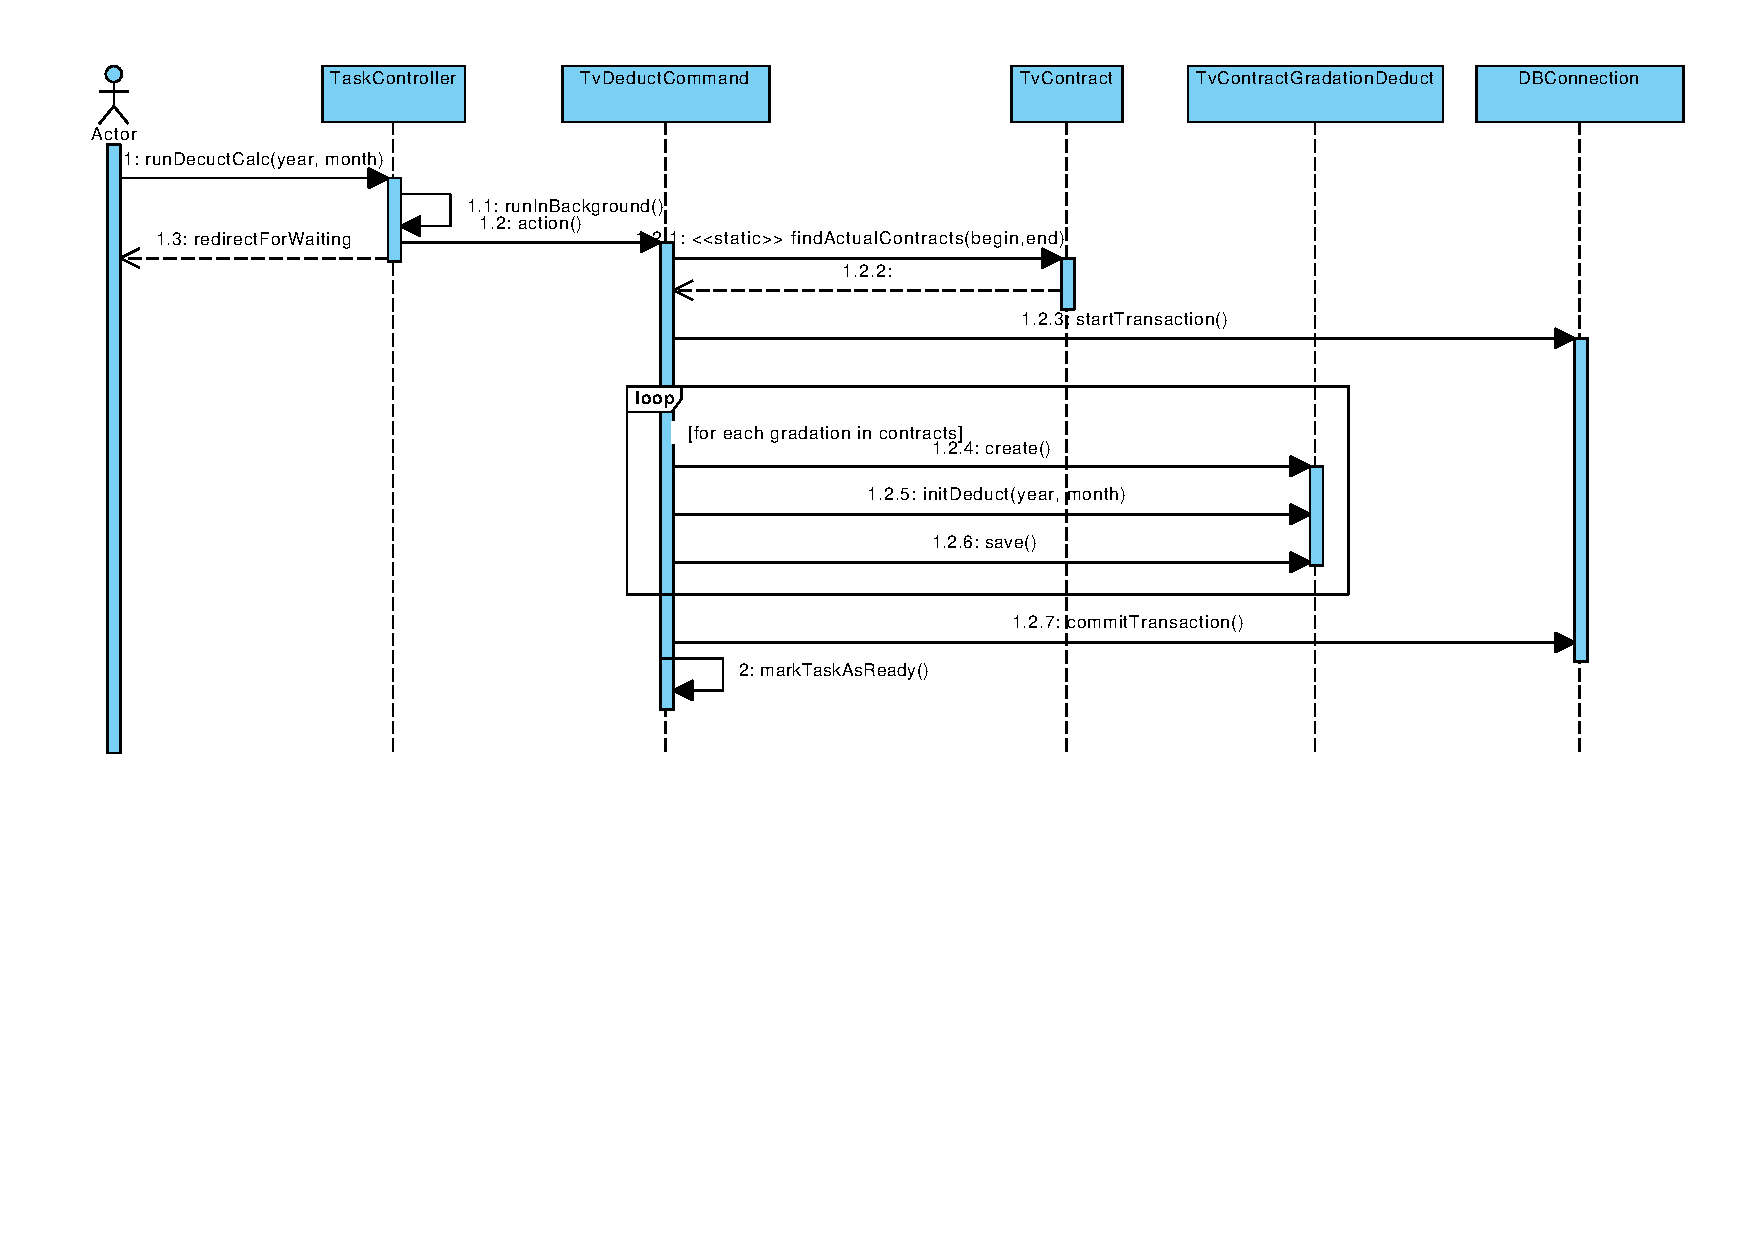
\includegraphics[scale=0.65, trim=10mm 80mm 0mm 10mm, clip]{../resources/uml/CalcDeduct.pdf}
\caption{Диаграмма последовательность для процесса расчета отчислений по Live}
\label{gr:calc_deduct}
\end{center} 
\end{figure}

В форме запуска расчета отчислений пользователь выбирает год и месяц, для которого
должны быть вычислены значения. После отправки формы запускается фоновая задача ``TvDeductCommand'',
в методе \textit{action()} которой происходит выборка актуальных договоров.

Непосредственно алгоритм расчета запускается в рамках транзакции СУБД, которая позволяет отменить уже внесенные 
в базу данных изменения в случае возникновения ошибки.

Для каждого объекта градации договоров создается соответствующий объект класса ``TvContractGratadionDeduct''
(отчисление по градации) и вызывается метод \textit{initDeduct()}, в котором и происходит расчет по градации
в соответствие с алгоритмом, описанным в \ref{live:deducts}.
